\section{Experiments}
\label{experiments}
This section evaluates the accuracy and performance of each model developed in the previous section.

\subsection{Accuracy}
\label{experiments.accuracy}
Using the test data that was set aside at the very beginning, each model was evaluated for base accuracy. These accuracies are 
presented in the following table, along with the equivelant scores on the training data.

\begin{figure} [!h]
    \centering
    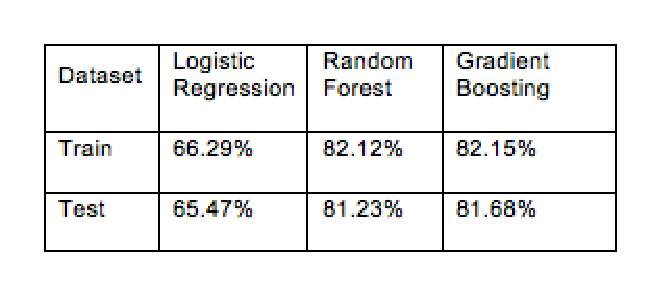
\includegraphics[scale=0.5]{figs/acc.eps}
    \label{table:acc}
    \caption{Accuracy of Each Classifier on Training \& Test Data}
\end{figure}

Accuracy only slighly decreased from training to test data, which means that overfitting was well-mitigated. To get a more 
granular understanding of the accuracy of each model, the \emph{confusion matrix} for each is shown next.


\begin{figure}[!h]
    \centering
    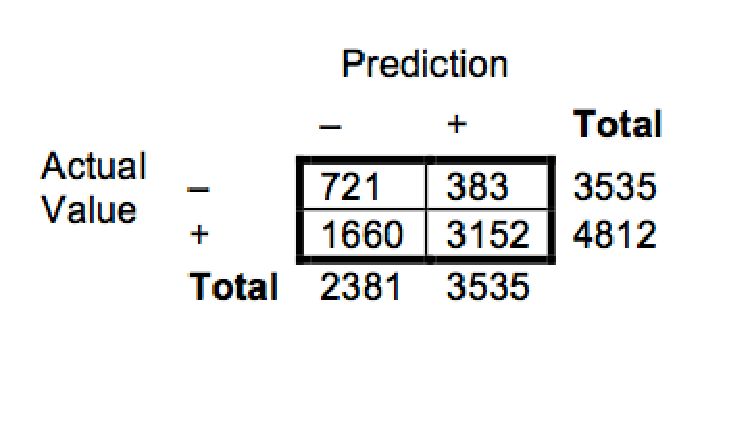
\includegraphics[scale=0.5]{figs/lr_conf.eps}
    \label{table:lr_conf}
    \caption{\textbf{Confusion Matrix for Logistic Regression}}
\end{figure}

\begin{figure}[!h]
    \centering
    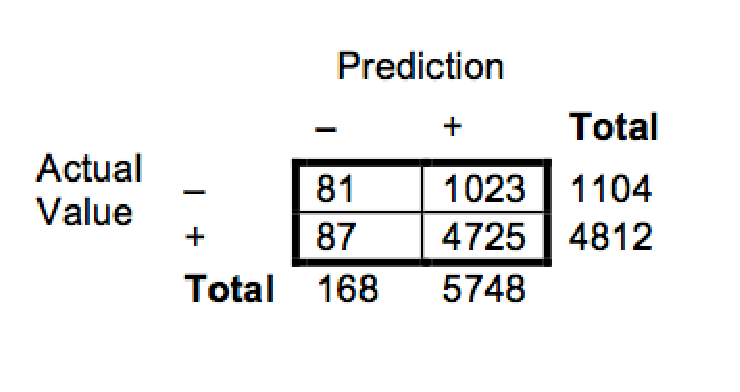
\includegraphics[scale=0.5]{figs/rf_conf.eps}
    \label{table:rf_conf}
    \caption{\textbf{Confusion Matrix for Random Forest}}
\end{figure}

\begin{figure}[!h]
    \centering
    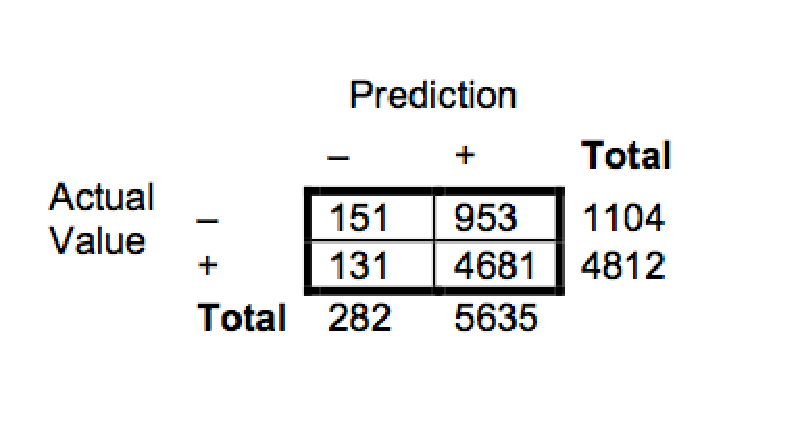
\includegraphics[scale=0.5]{figs/gb_conf.eps}
    \label{table:gb_conf}
    \caption{\textbf{Confusion Matrix for Gradient Boosting}}
\end{figure}

The confusion matrix shows false positives (fully paid loans that was predicted to default) in the upper-right quadrant and false 
negatives (defaulted loans that were predicted to be paid off) in the lower-left. The logistic regression model seems to 
be getting many more false positives than false negative, while the reverse is true in the two ensemble models. 
If using the classifier to select notes for investment, false negatives are a much more tolerable form of error than false
positives, as the former is an opportunity for profit missed, while the latter is actual capital lost (most people are more
disturbed by losing money than they are excited about making it). Taking this into account, both ensemble models are performing
even better than the logistic regression model, with the random forest model coming out slightly ahead of the gradient boosting 
one.

\subsection{Returns}
\label{experiments.returns}
Although it is important to evaluate the models' accuracy, the key consideration is how well each performs the function 
they were built for: maximizing returns. As stated earlier, Lending Club claims that every investor who has purchased 
800 notes (\$20,000 worth) has experienced positive returns, with 94\% greater than 6\%. Fig. 6 shows a 
more granular breakdown.


\begin{figure}[!h]
    \centering
    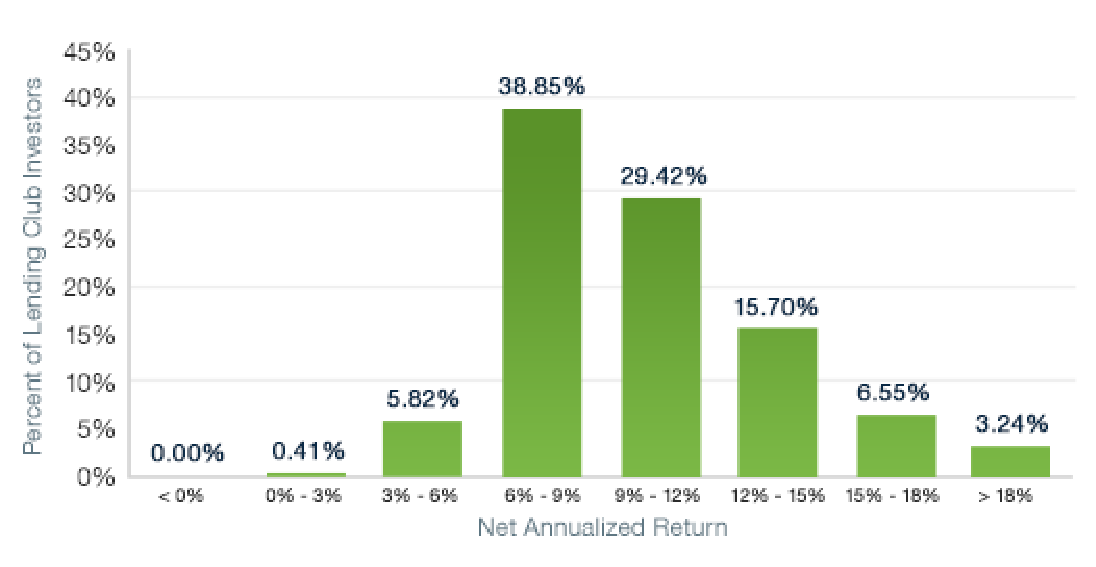
\includegraphics[scale=0.5]{figs/lc_stats.eps}
    \label{fig:lc_stats}
    \caption{\textbf{Distribution of Investor Returns (800+ Notes)}}
\end{figure}

For a classifier to be considered successful, it should be able to achieve greater returns than the general diversification tactic
that can be assumed to be in use by the average Lending Club investor.

The models created in this paper work by taking processed loan features as input and outputting the probability of that loan
defaulting. Though definitely useful, this is not exactly the same as reading all available loan data and picking the loans 
with the greatest likely returns. Therefore, two models of `best performance' are chosen and used for note selection. 
The first is to simply invest in the loans with the highest probability of becoming fully repaid. This would be expected to work
quite well if the models did not overfit the training data too much. It is also the \emph{safer} option, as it only tries
to pick successful notes and does not take into account the return. The second option is to pick notes with the highest 
\emph{expected utility}, which this paper will define as the probability of a note's success multiplied by the return it would achieve
if successful. For comparison purposes, and because diversification is generally a good thing, these metrics will be used to 
select the `best' 800 loans and evaluate their total performance if one note were purchased from each. To evaluate performance,
the Amount Repaid (which was set aside earlier) is divided by the Amount Funded and converted to a percentage. This percentage 
is averaged across all loans to obtain the total percent return on investment. The following table summarizes the results. 


\begin{figure}[!h]
    \centering
    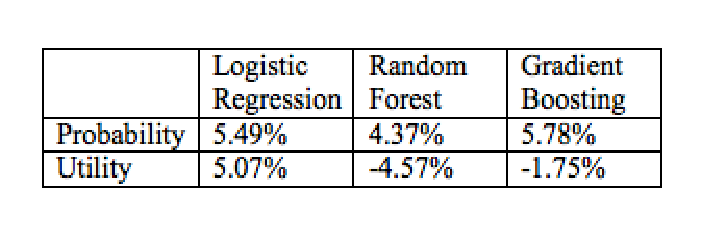
\includegraphics[scale=0.5]{figs/returns.eps}
    \label{table:returns}
    \caption{\textbf{Percent Returns for Each Classifier Maximizing Success Probability and Utility}}
\end{figure}

The results are clearly disappointing. Logistic regression, the intended baseline, ends up achieving better results than 
random forest when maximizing success probability, and only does slightly worse than gradient boosting. When maximizing 
utility, it is the clear winner. This could be because the function trained on is not exactly what is being tested here. 
Being a simpler model, the logistic regression model could have learned general relationships between features that are 
useful in other contexts, while the more sophisticated models learned a more complex, and therefore more brittle classification 
function that generalizes poorly to other tasks. In either case, each model perfromed worse than over 90\% of investors 
with the same number of notes! It would seem that the best strategy is the one that most ivestors are using, rather than 
any model developed in this paper.
